\documentclass[border=6pt]{standalone}
\usepackage[T1]{fontenc}
\usepackage{amsmath, amssymb}
\usepackage{tikz}
\usetikzlibrary{positioning, shapes.geometric, arrows.meta, fit,
                backgrounds, calc}

% --------------------------------------------------- Farben
\definecolor{physfill}{HTML}{DCE9F5}   % optische / physikalische Schritte
\definecolor{physline}{HTML}{2C5F8A}
\definecolor{ctrlfill}{HTML}{EFEFEF}   % Ablaufsteuerung
\definecolor{ctrlline}{HTML}{707070}
\definecolor{decfill} {HTML}{FBEBD2}   % Verzweigungen
\definecolor{decline} {HTML}{B07B23}
\definecolor{loopcol} {HTML}{8C8C8C}   % Rueckwaerts-Kanten

\begin{document}
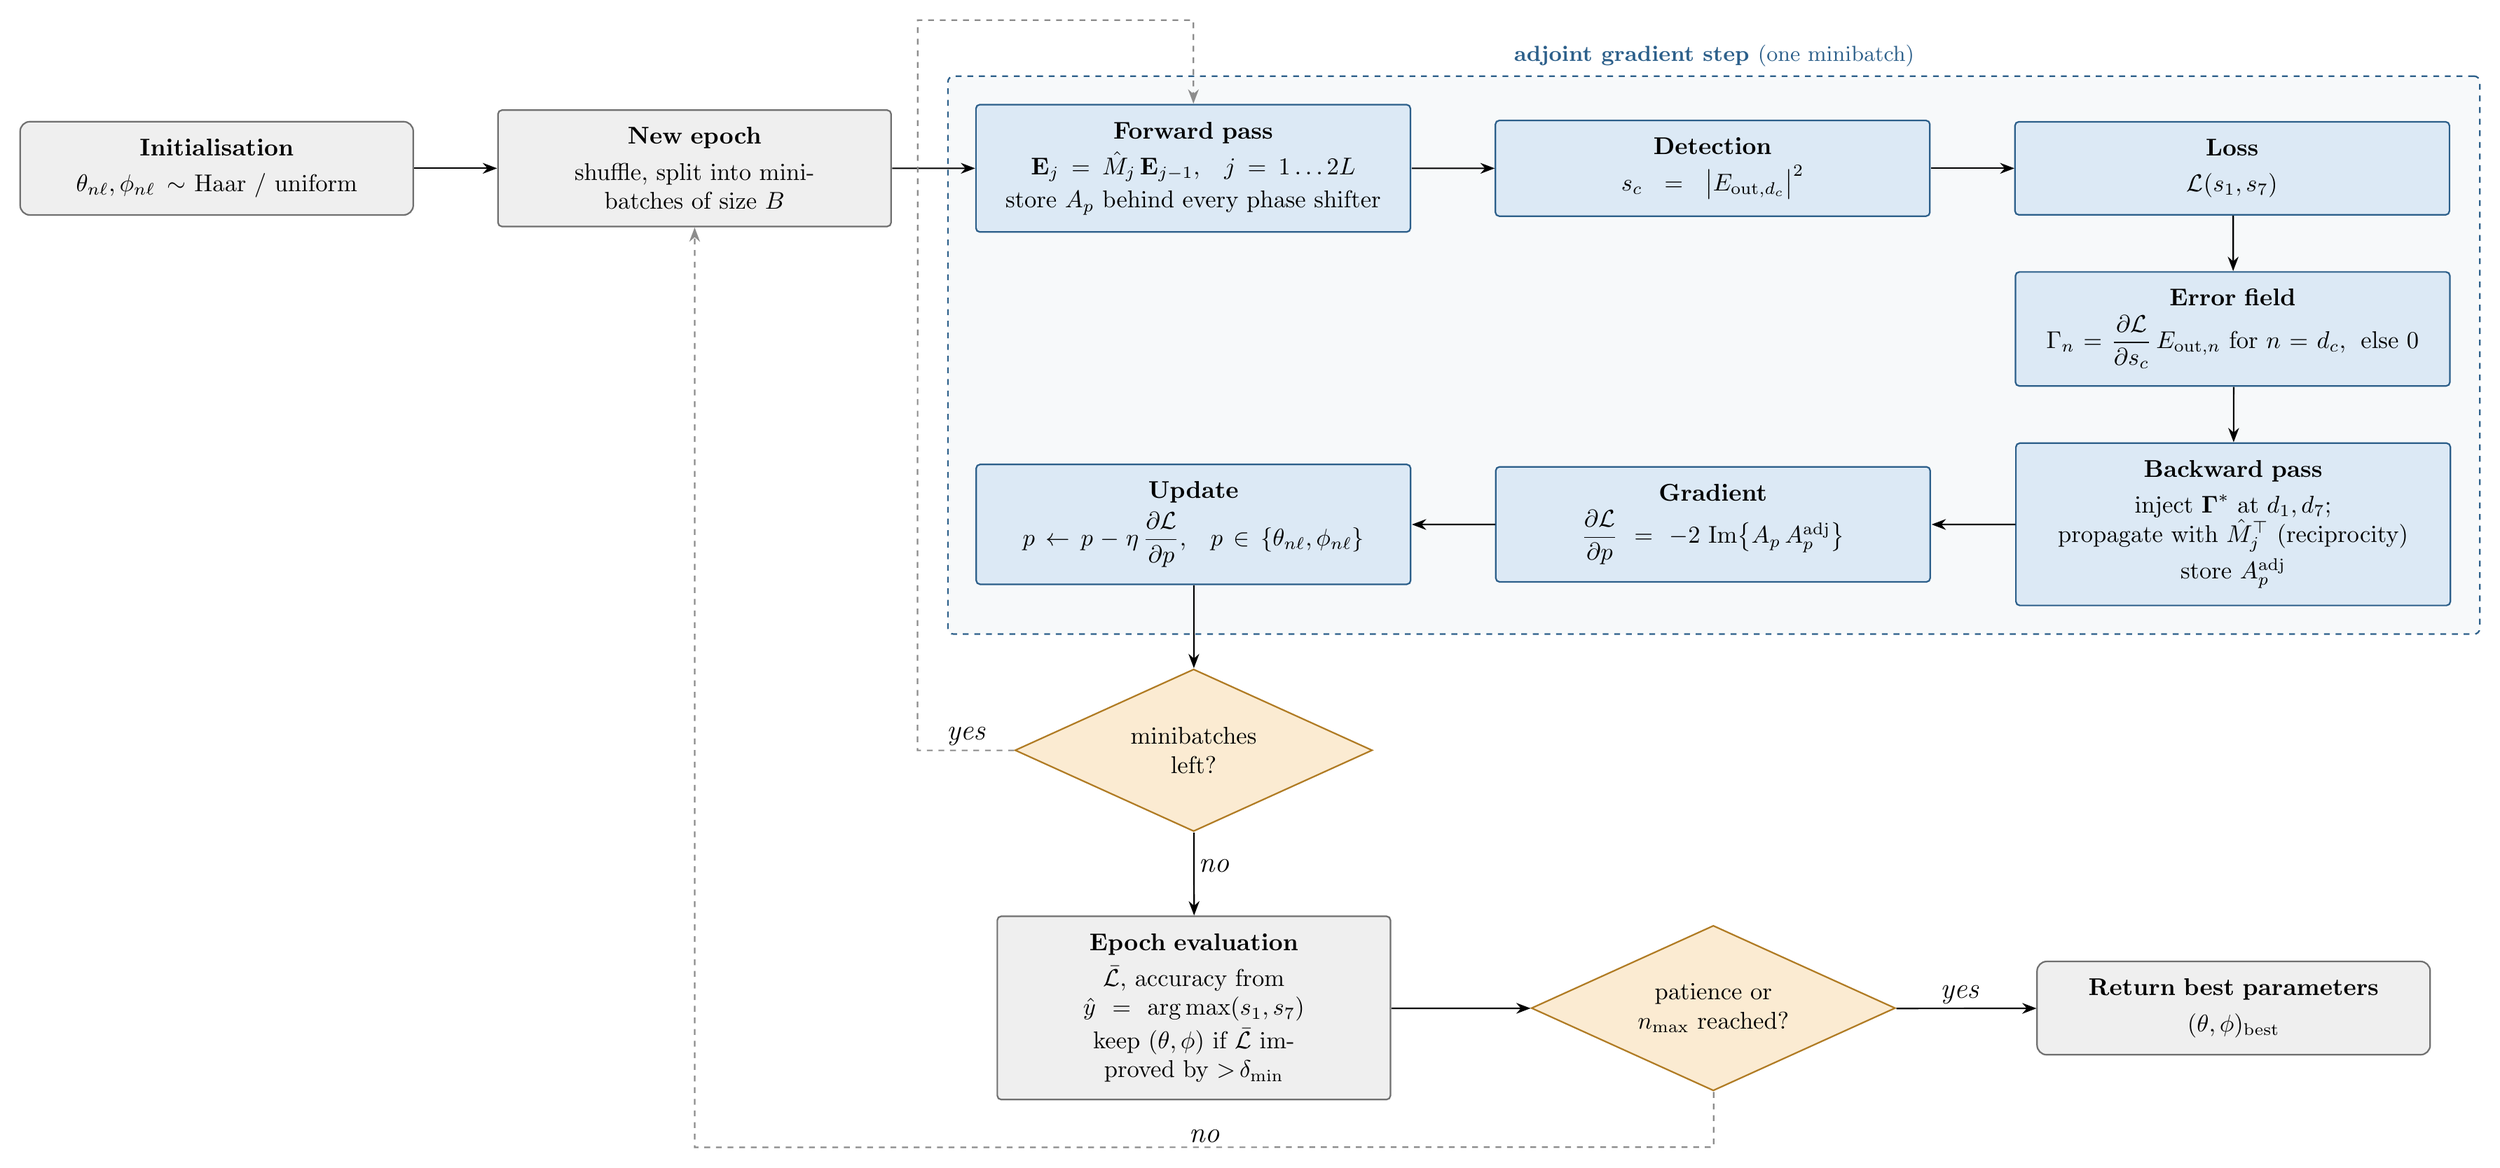
\begin{tikzpicture}[
    scale=1.25, transform shape, % Skaliert das gesamte Diagramm proportional
    font=\normalsize, % Schrift um ca. 2pt vergrößert
    node distance = 10mm and 12mm, % Vertikaler und horizontaler Abstand
    base/.style = {rectangle, rounded corners=2pt, draw, thick,
                   minimum height=12mm, text width=58mm, align=center,
                   inner sep=2.5mm},
    phys/.style = {base, fill=physfill, draw=physline},
    ctrl/.style = {base, fill=ctrlfill, draw=ctrlline, text width=52mm},
    term/.style = {base, rounded corners=5pt, fill=ctrlfill, draw=ctrlline,
                   text width=52mm},
    dec/.style  = {diamond, aspect=2.2, draw, thick, fill=decfill,
                   draw=decline, align=center, inner sep=0.5mm,
                   text width=34mm},
    flow/.style = {-{Stealth[length=2.6mm]}, thick},
    loop/.style = {-{Stealth[length=2.6mm]}, thick, draw=loopcol, dashed},
    lbl/.style  = {font=\large\itshape, inner sep=1.5pt} % Labels leicht vergrößert
  ]

% =========================================================================
%  Horizontales Layout: Reihe 1 (Forward Flow & Init)
% =========================================================================
\node[term] (init) {\textbf{Initialisation}\\[1mm]
   $\theta_{n\ell},\phi_{n\ell}\sim$ Haar / uniform};

\node[ctrl, right=of init] (shuf) {\textbf{New epoch}\\[1mm]
   shuffle, split into minibatches of size $B$};

\node[phys, right=of shuf] (fwd) {\textbf{Forward pass}\\[1mm]
   $\mathbf{E}_{j}=\hat{M}_{j}\,\mathbf{E}_{j-1}$,\quad $j=1\dots2L$\\[0.6mm]
   store $A_p$ behind every phase shifter};

\node[phys, right=of fwd] (det) {\textbf{Detection}\\[1mm]
   $s_c=\bigl|E_{\mathrm{out},d_c}\bigr|^{2}$\\[0.6mm]};

\node[phys, right=of det] (loss) {\textbf{Loss}\\[1mm]
   $\mathcal{L}(s_1,s_7)$};

% =========================================================================
%  Reihe 2 und 3: Der physikalische Rückweg (U-Form nach unten)
% =========================================================================
\node[phys, below=8mm of loss] (gam) {\textbf{Error field}\\[1mm]
   $\Gamma_n=\dfrac{\partial\mathcal{L}}{\partial s_c}\,E_{\mathrm{out},n}$
   for $n=d_c$,\; else $0$};

\node[phys, below=8mm of gam] (bwd) {\textbf{Backward pass}\\[1mm]
   inject $\boldsymbol{\Gamma}^{*}$ at $d_1,d_7$; \\propagate with
   $\hat{M}_{j}^{\top}$ (reciprocity)\\[0.6mm]
   store $A_p^{\mathrm{adj}}$};

\node[phys] (grad) at (det |- bwd) {\textbf{Gradient}\\[1mm]
   $\dfrac{\partial\mathcal{L}}{\partial p}
    =-2\,\operatorname{Im}\bigl\{A_p\,A_p^{\mathrm{adj}}\bigr\}$};

\node[phys] (upd) at (fwd |- bwd) {\textbf{Update}\\[1mm]
   $p\leftarrow p-\eta\,\dfrac{\partial\mathcal{L}}{\partial p}$,\quad
   $p\in\{\theta_{n\ell},\phi_{n\ell}\}$};

% =========================================================================
%  Reihe 4 und 5: Ablaufsteuerung (Minibatches und Epochen)
% =========================================================================
\node[dec, below=12mm of upd] (dbatch) {minibatches\\ left?};

\node[ctrl, below=12mm of dbatch] (eval) {\textbf{Epoch evaluation}\\[1mm]
   $\bar{\mathcal{L}}$, accuracy from
   $\hat{y}=\arg\max(s_1,s_7)$\\[0.6mm]
   keep $(\theta,\phi)$ if
   $\bar{\mathcal{L}}$ improved by ${>}\,\delta_{\min}$};

\node[dec] (dstop) at (grad |- eval) {patience or\\ $n_{\max}$ reached?};

\node[term] (fin) at (bwd |- eval) {\textbf{Return best parameters}\\[1mm]
   $(\theta,\phi)_{\mathrm{best}}$};

% =========================================================================
%  Hintergrundbox für den physikalischen Block
% =========================================================================
\begin{scope}[on background layer]
  \node[draw=physline, dashed, thick, rounded corners=3pt,
        inner sep=5mm, fill=physline!4,
        fit=(fwd)(det)(loss)(gam)(bwd)(grad)(upd)] (stepbox) {};
\end{scope}
\node[anchor=south, font=\small\bfseries, text=physline]
      at (stepbox.north)
      {adjoint gradient step \textnormal{(one minibatch)}};

% =========================================================================
%  Kanten und Verbindungen
% =========================================================================
\draw[flow] (init) -- (shuf);
\draw[flow] (shuf) -- (fwd);
\draw[flow] (fwd)  -- (det);
\draw[flow] (det)  -- (loss);
\draw[flow] (loss) -- (gam);
\draw[flow] (gam)  -- (bwd);
\draw[flow] (bwd)  -- (grad);
\draw[flow] (grad) -- (upd);
\draw[flow] (upd)  -- (dbatch);

% Loop: dbatch(yes) -> fwd 
% Exaktes Routing durch die Lücke zwischen 'shuf' und 'fwd'
\draw[loop] (dbatch.west) -- ++(-14mm,0) node[lbl, above, pos=0.5] {yes} coordinate (gap_up) 
      -- (gap_up |- stepbox.north) -- ++(0, 8mm) coordinate (top_line)
      -- (fwd.north |- top_line) -- (fwd.north);

\draw[flow] (dbatch.south) -- node[lbl, right, pos=0.4] {no} (eval.north);
\draw[flow] (eval) -- (dstop);

% Loop: dstop(no) -> shuf
% Exaktes Routing am unteren Rand entlang
\draw[loop] (dstop.south) -- ++(0,-8mm) coordinate (bot) 
      -- (bot -| shuf.south) node[lbl, above, pos=0.5] {no} 
      -- (shuf.south);

\draw[flow] (dstop) -- node[lbl, above, pos=0.45] {yes} (fin);

\end{tikzpicture}
\end{document}